\begin{apendicesenv}

\partapendices

\chapter{Members of GPP/MDS team}
\label {sec:apendice_a}

The following students were the direct responsible for developing the first version of the platform. They are students of the courses \textit{M\'etodos de Desenvolvimento de Software} and \textit{Gest\~ao de Portfolios e Projetos} ministered by Professor Carla Silva Rocha Aguiar.

\begin{itemize}
\item Arthur Temporim
\item Artur Bersan
\item Eduardo Nunes
\item Ícaro Pires de Souza Aragão
\item João Robson
\item Letícia de Souza
\item Marcelo Ferreira
\item Matheus Miranda
\item Rafael Bragança
\item Thiago Ribeiro Pereira
\item Varley Santana Silva
\item Victor Leite
\item Vinicius Ferreira Bernardo de Lima
\end{itemize}

\chapter{Selected games}
\label {sec:selected_games}

This appendix shows the authors, year of publication, quantity of players, genre and description, whenever possible, of each selected game for this first part of the project.

\section{Jack the Janitor}
\label {sec:jack_the_janitor}

\begin{itemize}
\item[] \textbf{Authors:} Athos Ribeiro, Alexandre Barbosa, Mateus Furquim, Átilla Gallio
\item[] \textbf{Year:} 1/2013
\item[] \textbf{Genre:} Puzzle, platform
\item[] \textbf{\# Players:} Single player
\item[] \textbf{Description: \footnote{Available on the game repository: https://github.com/fgagamedev/Jack-the-Janitor}} Jack, The Janitor is a puzzle game where the player controls Jack, a school's janitor who must organize the school's warehouse. Jack can push boxes to the left or to the right and jump boxes.

When Jack fills an entire row with boxes, they disappear from the screen and go to a small window on the right side of he screen called the closet.

The closet shows how Jack organized the rows of boxes. When similar boxes are combined in the closet, Jack gets extra points and some power ups (to be implemented).

The game ends if a falling box hits Jack or if the closet gets full.

\end{itemize}

\section{Emperor vs Aliens}
\label {sec:emperor}

\begin{itemize}
\item[] \textbf{Authors:} Leonn Ferreira, Luis Gustavo
\item[] \textbf{Year:} 2/2012
\item[] \textbf{Genre:} Tower defense
\item[] \textbf{\# Players:} Single player
\end{itemize}

\section{Ninja Siege}
\label {sec:ninja_siege}

\begin{itemize}
\item[] \textbf{Authors:} Tiago Gomes Pereira, Matheus Fonseca, Charles Oliveira, Pedro Zanini
\item[] \textbf{Year:} 2/2012
\item[] \textbf{Genre:} Tower defense
\item[] \textbf{\# Players:} Single player
\item[] \textbf{Description:} The ninja academy is being raided and you have to defend it.
\end{itemize}


\section{Space Monkey}
\label {sec:space_monkey}

\begin{itemize}
\item[] \textbf{Authors:} Victor Cotrim
\item[] \textbf{Year:} 2/2012
\item[] \textbf{Genre:} Tower defense
\item[] \textbf{\# Players:} Single player
\item[] \textbf{Description:} Monkeys are attacking your home planet. They come in waves and you have to get rid of them all.
\end{itemize}

It's interest to notice that, by this time, the students of \textit{Introdu\c{c}\~ao aos Jogos Eletr\^onicos} didn't have designers with them in the team. Figure \ref{fig:space_monkey} shows that, given the complexity of developing a game, sometimes the artwork was not a priority. This is also one of the games that didn't run properly after the compilation.

\begin{figure}[h!]
\centering
\fbox{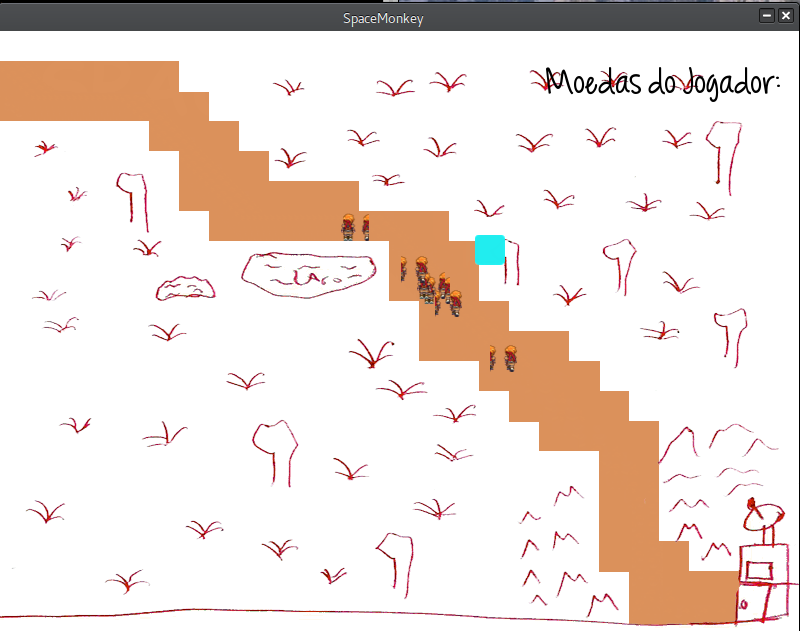
\includegraphics[width=300px,height=\textheight,keepaspectratio]{prints/space_bug1}}
\caption{Space Monkey}
\label{fig:space_monkey}
\end{figure}


\section{War of the Nets}
\label {sec:war}

\begin{itemize}
\item[] \textbf{Authors:} Matheus Faira, Lucas Kanashiro, Luciano Prestes, Lucas Moura
\item[] \textbf{Year:} 2/2013
\item[] \textbf{Genre:} Turn Based Strategy
\item[] \textbf{\# Players:} Multi player
\item[] \textbf{Description:} It is a turn based strategy (TBS), where the objective is to construct a network from the base to a right point, faster than your enemy. You also can destroy his network with bombs, or infiltrate it with spies.

\end{itemize}

\section{Post War}
\label {sec:post_war}

\begin{itemize}
\item[] \textbf{Authors:} Bruno de Andrade, Jonathan Rufino, Yago Regis
\item[] \textbf{Year:} 2/2013
\item[] \textbf{Genre:} Turn Based Strategy
\item[] \textbf{\# Players:} Multi player
\end{itemize}

\section{Ankhnowledge}
\label {sec:ankh}

From the games developed before the time the course was taught in conjunction with the students from \textit{Darcy Ribeiro}, this is one of the prettiest and most pleasant games to play. Because one of the students is a software developer and designer, the user interface was very well drawn as seen in Figure \ref{fig:ankh}.

\begin{figure}[h!]
\centering
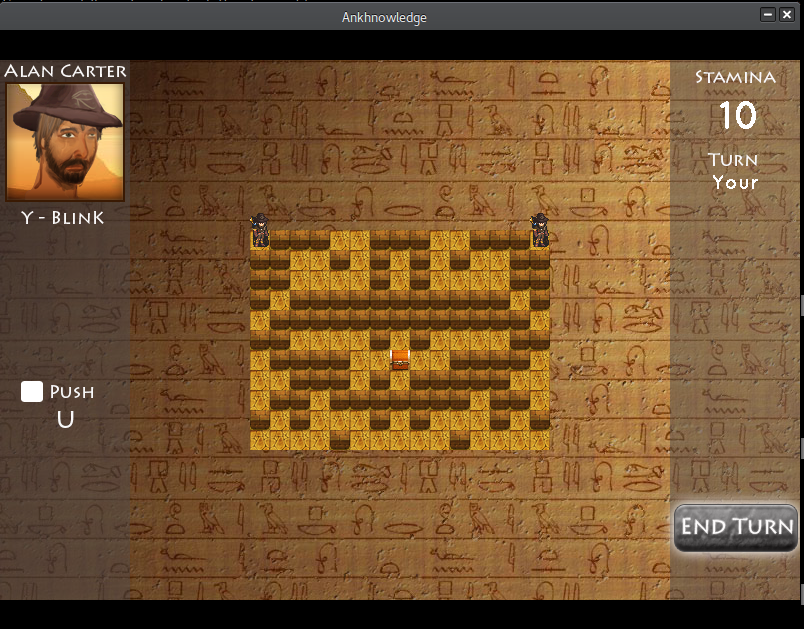
\includegraphics[width=350px,height=\textheight,keepaspectratio]{prints/ankh_cut}
\caption{Ankhnowledge}
\label{fig:ankh}
\end{figure}

\begin{itemize}
\item[] \textbf{Authors:} Arthur del Esposte, Alex Campelo, Atilla Gallio
\item[] \textbf{Year:} 2/2013
\item[] \textbf{Genre:} Turn Based Strategy
\item[] \textbf{\# Players:} Multi player
\end{itemize}


\section{Last World War}
\label {sec:last_world_war}


\begin{itemize}
\item[] \textbf{Authors:} Gabriela Navarro
\item[] \textbf{Year:} 2/2013
\item[] \textbf{Genre:} Turn Based Strategy
\item[] \textbf{\# Players:} Multi player
\end{itemize}


\section{Kays against the World}
\label {sec:kays}


\begin{itemize}
\item[] \textbf{Authors:} Carlos Coelho, Bruno de Amorim Campos, Bruno Carbonell, Guilherme Fenterseifer, Fernando Tollendal, Lucas Sanginez, Victor Bednarczuk
\item[] \textbf{Year:} 1/2014
\item[] \textbf{Genre:} Platform
\item[] \textbf{\# Players:}
\end{itemize}


\section{Imagina na Copa}
\label {sec:imagina}

\begin{itemize}
\item[] \textbf{Authors:} Iago Mendes Leite, Jonathan Henrique Maia de Moraes, Luciano Henrique Nunes de Almeida, Inara Régia Cardoso, Renata Rinaldi, Lucian Lorens Ramos
\item[] \textbf{Year:} 1/2014
\item[] \textbf{Genre:} Platform
\item[] \textbf{\# Players:}
\end{itemize}

\section{Dauphine}
\label {sec:dauphine}

\begin{itemize}
\item[] \textbf{Authors:} Caio Nardelli, Simiao Carvalho
\item[] \textbf{Year:} 1/2014
\item[] \textbf{Genre:} Platform
\item[] \textbf{\# Players:} Single player
\item[] \textbf{Description:} A platforming/stealth game in a medieval fantasy setting, developed with SDL2.
\end{itemize}


\section{Terracota}
\label {sec:terracota}

\begin{itemize}
\item[] \textbf{Authors:} Álvaro Fernando, Macartur Sousa, Carlos Oliveira, André Coelho, Pedro Braga, Wendy Abreu, José de Abreu
\item[] \textbf{Year:} 1/2015
\item[] \textbf{Genre:} Adventure
\item[] \textbf{\# Players:} Single player
\end{itemize}

\section{7 Keys}
\label {sec:seven_keys}

\begin{itemize}
\item[] \textbf{Authors:} Paulo Markes, Bruno Contessotto Bragança Pinheiro, Lucas Rufino, Luis André Leal de Holanda Cavalcanti, Maria Cristina Monteiro de Oliveira, Guilherme Henrique Nunes Lopes
\item[] \textbf{Year:} 1/2015
\item[] \textbf{Genre:} Adventure
\item[] \textbf{\# Players:} Single player
\end{itemize}


\section{Babel}
\label {sec:babel}

\begin{itemize}
\item[] \textbf{Authors:} Álex Silva Mesquita, Jefferson Nunes de Sousa Xavier, Rodrigo Gonçalves, Vinícius Corrêa de Almeida, Heitor Campos, Max Von Behr, Aleph Telles de Andrade Casara, Washington Rayk
\item[] \textbf{Year:} 1/2015
\item[] \textbf{Genre:} Adventure
\item[] \textbf{\# Players:} Single player
\item[] \textbf{Description:} The mankind wanders the universe looking for a new habitable planet. They found an unknown planet with a big and strange tower.

The challenge is explore the tower and the planet and expand your resources, but be careful with the mysteries of this new planet.
\end{itemize}

\section{Strife of Mithology}
\label {sec:strife}

\begin{itemize}
\item[] \textbf{Authors:} Jônnatas Lennon Lima Costa, Marcelo Martins de Oliveira, Victor Henrique Magalhães Fernandes, Dylan Jefferson M. Guimarães Guedes
\item[] \textbf{Year:} 1/2016
\item[] \textbf{Genre:} Tower Defense
\item[] \textbf{\# Players:} Single player
\item[] \textbf{Description:} A 2d-isometric Tower Defense based on mythology.
\end{itemize}

\section{Traveling Will}
\label {sec:traveling}

\begin{itemize}
\item[] \textbf{Authors:} Jo\~ao Ara\'ujo, Vitor Araujo, Igor Ribeiro Duarte, Jo\~ao Paulo Busche da Cruz
\item[] \textbf{Year:} 1/2016
\item[] \textbf{Genre:} Platform, Runner
\item[] \textbf{\# Players:} Single player
\item[] \textbf{Description:} This game tells the story of Will, personification of the Will, trying to restore
\end{itemize}

This game has one of the most attractive user interfaces from the games packaged so far. The team that developed it was able to create a very good game, technically speaking, with engaging scenarios and soundtrack, because they had design and music students. A screen of the game running after compiling it with the building script is shown in Figure \ref{fig:traveling_will}.

\begin{figure}[h!]
\centering
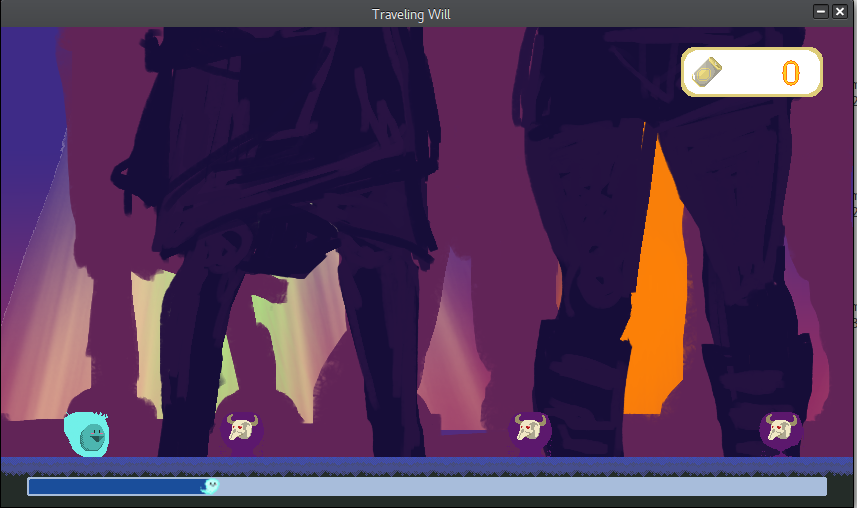
\includegraphics[width=300px,height=\textheight,keepaspectratio]{prints/travel_fase3}
\caption{Traveling Will}
\label{fig:traveling_will}
\end{figure}



\section{Deadly Wish}
\label {sec:deadly_wish}

\begin{itemize}
\item[] \textbf{Authors:} Lucas Mattioli, Victor Arnaud, Vitor Nere, Iago Rodrigues
\item[] \textbf{Year:} 1/2016
\item[] \textbf{Genre:} Battle Arena
\item[] \textbf{\# Players:} Single player
\end{itemize}
\end{apendicesenv}



